% ==============================================================
%	Introduction to LaTeX
%	Author: Fidele IRADUKUNDA
% ==============================================================

\documentclass[12pt]{article}	% Article layout with 12 pt text

% ==============================================================
%	PACKAGES
% ==============================================================
\usepackage{amsmath, amssymb}	% Equations and mathematical symbols
\usepackage{booktabs}	% Clean, professional table lines
\usepackage{graphicx}	% Insert images and figures

\usepackage[
	colorlinks=true,	% Show links as coloured text, not boxes
	linkcolor=black,	% Contents and cross-references in black
	citecolor=blue,	% Citations in blue
	urlcolor=blue	% Web addresses in blue
]{hyperref}	% Clickable links (always load last)

% ==============================================================
%	TITLE INFORMATION
% ==============================================================
\title{Introduction to LaTeX}	% Document title
\author{	% Author details (\\ starts a new line)
	Fidele IRADUKUNDA\\	% Full name
	Faculty of IT\\	% Faculty
	Adventist University of Central Africa\\	% Institution
	\texttt{niyongaboaristide17@gmail.com}	% Email in monospace font
}
\date{\today}	% Insert the current date automatically

% ==============================================================
%	DOCUMENT BODY
% ==============================================================
\begin{document}

	% ---------- Title page ----------
	\maketitle	% Print title, author and date
	\newpage	% Move to a new page

	% ---------- Table of contents ----------
	\tableofcontents	% Contents from headings (compile twice)
	\newpage	% Move to a new page

	% ---------- Abstract ----------
	\begin{abstract}	% Start of the abstract
		In this study, we present the Lebesgue integral ...
		We also introduce regression analysis and the structure
		of this document.
	\end{abstract}	% End of the abstract
	\newpage	% Move to a new page

	% ---------- Section 1: Introduction ----------
	\begin{section}{Introduction}	% Start of Section 1
		\label{sec:introduction}	% Name for referencing

		In this study, we use regression analysis to estimate the fair
		price on the financial market.

		As explained in Section~\ref{sec:methodology}, we will describe
		the methodology used in this study.

		The background of the study is discussed in
		Section~\ref{sec:background}, while the objectives are presented
		in Section~\ref{sec:objectives}.

		% ---------- Unordered list ----------
		\begin{itemize}	% Start of bullet list
			\item Monday
			\item Tuesday
			\item Wednesday
			\item Thursday
		\end{itemize}	% End of bullet list

		% ---------- Ordered list ----------
		\begin{enumerate}	% Start of numbered list
			\item Monday
			\item Tuesday
			\item Wednesday
			\item Thursday
		\end{enumerate}	% End of numbered list

		% ---------- Subsection 1.1: Background ----------
		\begin{subsection}{Background}	% Start of 1.1
			\label{sec:background}	% Name for referencing

			Background of the study ...

			For additional information about the study objectives,
			see Section~\ref{sec:objectives}.
		\end{subsection}	% End of 1.1

		% ---------- Subsection 1.2: Objectives ----------
		\begin{subsection}{Objectives}	% Start of 1.2
			\label{sec:objectives}	% Name for referencing

			Our objective is ...

			% ---------- Sub-subsection 1.2.1 ----------
			\begin{subsubsection}{General Objective}	% Start of 1.2.1
				\label{sec:general-objective}	% Name for referencing

				My general objective is ...
			\end{subsubsection}	% End of 1.2.1

			% ---------- Sub-subsection 1.2.2 ----------
			\begin{subsubsection}{Specific Objectives}	% Start of 1.2.2
				\label{sec:specific-objectives}	% Name for referencing

				The specific objectives are ...

				The general objective is presented in
				Section~\ref{sec:general-objective}, and the specific objectives
				are described in Section~\ref{sec:specific-objectives}.
			\end{subsubsection}	% End of 1.2.2

		\end{subsection}	% End of 1.2
	\end{section}	% End of Section 1

	% ---------- Section 2: Methodology ----------
	\begin{section}{Methodology}	% Start of Section 2
		\label{sec:methodology}	% Name for referencing

		Our methodology ...

		As introduced in Section~\ref{sec:introduction}, this section
		describes the methods used in the study.
	\end{section}	% End of Section 2

	\newpage	% Move to a new page

	% ---------- Section 3: Graphs ----------
	% ---------- Section 3: Graphs ----------
	\begin{section}{Graphs}	% Start of Section 3
		\label{sec:graphs}	% Name for referencing

		Figure~\ref{fig:graph1} shows the first graph of the study.	% Prints: Figure 1

		% ---------- Figure 1 ----------
		\begin{figure}[htbp]	% Start of the figure (h=here, t=top, b=bottom, p=own page)
			\centering	% Centre the graph on the page
			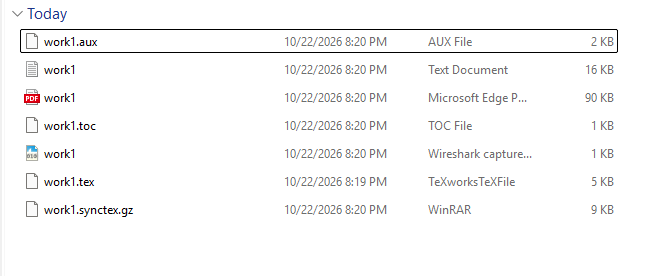
\includegraphics[width=0.8\textwidth]{Graph1.png}	% Insert Graph1.png at 80% of the text width
			\caption{Graph 1: description of what the graph shows}	% Caption below the graph
			\label{fig:graph1}	% Name for referencing (always after the caption)
		\end{figure}	% End of the figure
	\end{section}	% End of Section 3

\end{document}	% End of the document